%Plantilla basada en "Template for Masters / Doctoral Thesis" (plantilla disponible en writeLaTex) que subió LaTeXTemplates.com

\documentclass[11pt, oneside]{book}
\usepackage[paperwidth=17cm, paperheight=22.5cm, bottom=2.5cm, right=2.5cm]{geometry}
\usepackage{amssymb,amsmath,amsthm} %paquete para símbolo matemáticos
\usepackage[english]{babel}
\usepackage[utf8]{inputenc} %Paquete para escribir acentos y otros símbolos directamente
\usepackage{enumerate}
\usepackage{hhline}
\usepackage{graphicx}
\usepackage{float}
\usepackage{subcaption}
%\usepackage{subfig} %para poner subfiguras
%\usepackage{subcaption}
\graphicspath{{Figures/}{Figures/Plots}} %En qué carpeta están las imágenes
%\usepackage[nottoc]{tocbibind}
\usepackage[pdftex,
            pdfauthor={Carlos Miguel Patiño},
            pdftitle={Phenomenological Study of Heavy Neutrinos at the LHC, through high mass resonances, using the vector boson fusion technique},
            pdfsubject={Physics},
            pdfkeywords={PALABRAS CLAVE},
            pdfproducer={Latex con hyperref},
            pdfcreator={pdflatex}]{hyperref}



\begin{document}

%----------------------------------------------------------------------------------------
%	COMANDOS PERSONALIZADOS
%----------------------------------------------------------------------------------------

%SI TU TESIS TIENE TEOREMAS Y DEMOSTRACIONES, PUEDES DESCOMENTAR Y USAR LOS SIGUIENTES COMANDOS

%\renewcommand{\proofname}{Demostración}
%\providecommand{\norm}[1]{\lVert#1\rVert} %Provee el comando para producir una norma.
%\providecommand{\innp}[1]{\langle#1\rangle} 
%\newcommand{\seno}{\mathrm{sen}}
%\newcommand{\diff}{\mathrm{d}}

%\newtheorem{teo}{Teorema}[section] 
%\newtheorem{cor}[teo]{Corolario}
%\newtheorem{lem}[teo]{Lema}

%\theoremstyle{definition}
%\newtheorem{dfn}[teo]{Definición}

%\theoremstyle{remark}
%\newtheorem{obs}[teo]{Observación}

%\allowdisplaybreaks


%----------------------------------------------------------------------------------------
%	PORTADA
%----------------------------------------------------------------------------------------

\title{Heavy Neutrino VBF Analysis} %Con este nombre se guardará el proyecto en writeLaTex

\begin{titlepage}
\begin{center}

\textsc{\Large Universidad de los Andes}\\[3em]

\textsc{\large Faculty of Science}\\[1em]

\textsc{\large Physics Department} \\[1em]

%Figura
\begin{figure}[H]
\begin{center}

\includegraphics[scale = 0.4]{logo-uniandes.png}
\end{center}
\end{figure}

\vspace{0.5em}

\textsc{\huge \textbf{Phenomenological Study of Heavy Neutrinos at the LHC, through high mass resonances, using the vector boson fusion technique}}\\[4em]

%\textsc{\large Tesis}\\[1em]


%\textsc{que para obtener el título de}\\[1em]

%\textsc{TÍTULO  VAS A OBTENER}\\[1em]

\textsc{Author:}\\[1em]

\textsc{\Large Carlos Miguel Patiño}\\[1em]

\textsc{\large Advisor: Carlos Andrés Flórez}

\end{center}

\vspace*{\fill}
\textsc{Bogotá D.C. \hspace*{\fill} 2017}

\end{titlepage}


%----------------------------------------------------------------------------------------
%	DECLARACIÓN
%----------------------------------------------------------------------------------------

%\thispagestyle{empty}
%\vspace*{\fill}
%\begingroup
%``Con fundamento en los artículos 21 y 27 de la Ley Federal del Derecho de Autor y como titular de los derechos moral y patrimonial de la obra titulada ``\textbf{TÍTULO DE LA TESIS}'', otorgo de manera gratuita y permanente al Instituto Tecnológico Autónomo de México y a la Biblioteca Raúl Bailléres Jr., la autorización para que fijen la obra en cualquier medio, incluido el electrónico, y la divulguen entre sus usuarios, profesores, estudiantes o terceras personas, sin que pueda percibir por tal divulgación una contraprestación''.

%\centering

%\hspace{3em}

%\textsc{AUTOR}

%\vspace{5em}

%\rule[1em]{20em}{0.5pt} % Línea para la fecha

%\textsc{Fecha}
 
%\vspace{8em}

%\rule[1em]{20em}{0.5pt} % Línea para la firma

%\textsc{Firma}

%\endgroup
%\vspace*{\fill}


%----------------------------------------------------------------------------------------
%	DEDICATORIA
%----------------------------------------------------------------------------------------

%\pagestyle{empty}
\frontmatter

%\chapter*{}
%\begin{flushright}
%\textit{DEDICATORIA}
%\end{flushright}


%----------------------------------------------------------------------------------------
%	AGRADECIMIENTOS
%----------------------------------------------------------------------------------------

%\chapter*{Agradecimientos}
%\markboth{AGRADECIMIENTOS23}{AGRADECIMIENTOS} % encabezado 

%¡Muchas gracias a todos!


%----------------------------------------------------------------------------------------
%	PREFACIO
%----------------------------------------------------------------------------------------

%\chapter*{Prefacio}

%\pagestyle{plain}
%\markboth{PREFACIO23}{PREFACIO} % encabezado 

%PUEDEN QUITAR ESTA PARTE


%----------------------------------------------------------------------------------------
%	TABLA DE CONTENIDOS
%---------------------------------------------------------------------------------------

\tableofcontents

\listoffigures


%----------------------------------------------------------------------------------------
%	TESIS
%----------------------------------------------------------------------------------------
\mainmatter %empieza la numeración de las páginas
\pagestyle{headings}

%  Incluye los capítulos en el folder de capítulos

\chapter{Introduction}

The standard model (SM) gathers the entire understanding about fundamental particles and their interactions. Although the model has successfully explained various physical phenomena observed experimentally, there are still multiple unanswered questions concerning particle physics. For example, experiments \cite{Detectores} have shown that accelerator and reactor, solar, and atmospheric neutrinos have mass by proving the existence of neutrino oscillations. The fact that there are neutrino oscillations contradicts the SM, because this model precits that the neutrinos are massless. Some specific experiments for each neutrino category are: Super-Kamiokande \cite{Super-Kamiokande} for solar and atmospheric neutrino oscillations, KamLAND \cite{KamLAND} for reactor neutrinos, and K2K \cite{K2K} for accelerator neutrino oscillations \cite{Experimentos}. An additional open question about neutrinos is the fact that only neutrinos with left helicity have been observed. Helicity is defined as the projection of the particle's momentum vector over its spin direction. Only neutrinos with spin anti-parallel to its linear momentum have been observed.

In order to provide neutrinos with mass, several theories that extend the predictions of the SM have been proposed. One of the most known models is the "see-saw" or balance mechanism \cite{See-saw}. The see-saw mechanism includes three sub-models that provide mass to neutrinos. In this model, $\Phi = (\phi^{+}, \phi^{0})^{T}$ is the doublet associated with the SM Higgs Boson and $L_{l}$ the representation of a doublet field associated with the lepton number +1. In the type I see-saw mechanism the product between $L_{l}$ and $\Phi$ results in a fermionic singlet state. In the type II see-saw mechanism, the product between the two elements forms a scalar triplet. Finally, the product between $L_{l}$ and $\Phi$ in the type III sub-model results in a fermionic triplet state. Besides the see-saw mechanism, other models propose the existence of neutrinos with high mass and right helicity. If this kind of neutrinos are observed, the left and right symmetry in the SM would be restored and the mechanism by which the neutrinos acquire mass would be explained.

Heavy neutrinos searches have been conducted in experiments LEP \cite{LEP}, CMS and ATLAS \cite{CMS ATLAS}, but none of these collaborations has proved that heavy neutrinos exist. In order to understand heavy neutrino searches it is necessary to define the concept of jet. A jet at phenomenological level is defined as a quark or a gluon. In high energies experimental physics, a jet is defined as a collection of particles resulting from the fragmentation of quarks or gluons. Searches at CMS and ATLAS have focused in final states with associated leptons and jets. Figure \ref{fig: W} shows a Feynman diagram of the production of a heavy neutrino mediated by a W boson with left or right helicity. The final state for this process has two leptons ($\mu$ or $\tau$) and two jets.

\begin{figure}[H]
\centering
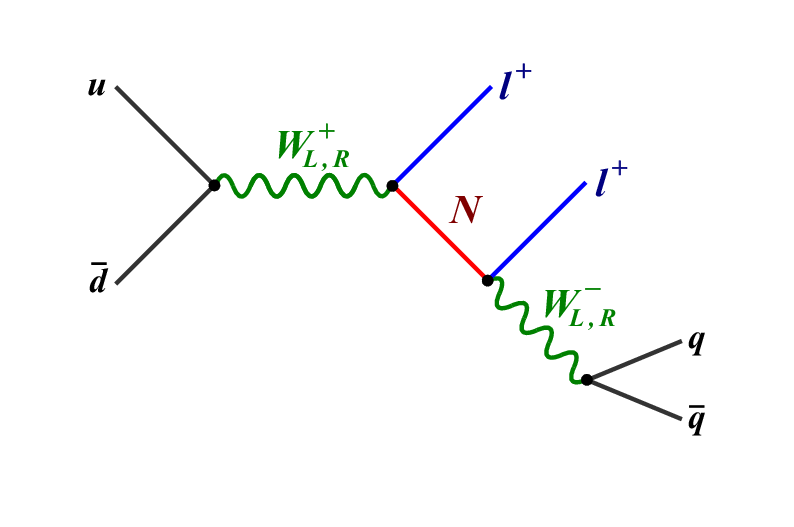
\includegraphics[width=\linewidth]{Figures/Feynman_W.png}
\caption{Feynman diagram of heavy neutrino production. (Taken from \cite{CMS ATLAS})}
\label{fig: W}
\end{figure}

The main objective of this monograph is to perform a phenomenological study about the feasibility of conducting an experimental analysis for the detection of heavy neutrinos in the Large Hadron Collider (LHC) using a technique known as vector boson fusion (VBF). This technique has been recently used in the LHC \cite{VBF Search} in searches for new physics. In high energy physics, the bosons $W^{\pm}$, $Z^{0}$ and $\gamma$ are known as vector bosons. The process of vector boson fusion occurs through an electroweak interaction of associated quarks with the LHC proton beams. In the analysis, the production of heavy neutrinos is considered through the decay of a high mass hypothetical resonance known as $Z^{'}$ (shown in the Feynman diagram of Figure \ref{fig: VBF}). This high mass resonance comes from the vector boson fusion process.

\begin{figure}[H]
\centering
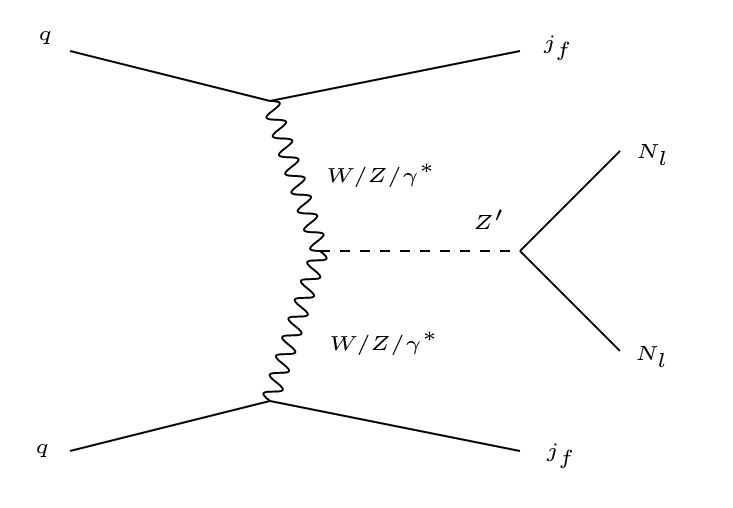
\includegraphics[scale = 0.65]{Figures/Feynman_VBF.JPG}
\caption{Feynman diagram of VBF process.}
\label{fig: VBF}
\end{figure}

The production of the heavy neutrino consists in the interaction of two quarks associated to the protons colliding in the beam. The protons emit vector bosons that produce a heavy resonance when they fuse. The heavy resonance decays afterwards producing the heavy neutrinos ($N_{l}$): $pp \rightarrow jj Z^{'} \rightarrow jj N_{l}N_{l}$.

The VBF topology consists in requiring two highly energetic jets in the longitundinal region of the detector and in opposite hemispheres thereof. It has been shown that by requiring this type of event, the noise level (background) is reduced considerably in regions of difficult study in searches of new physics.


In order to conduct the analysis, it is important to simulate signal and background processes and to perform a detailed physical study of the variables that allow to distinguish signal for experimental noise. It is necessary to use a cuantitative estimator commonly known as figure of merit to determine optimal cuts in the mentioned variables. The latter with the objective of reducing the amount of experimental noise by finding the optimal cuts in the relevant variables. For this particular analysis, the significance formula that will be used is the one shown in Equation 1, where $S$ is the significance, $N(s)$ is the number of signal events, and $N(B)$ is the number of background events.

\begin{equation}
    S = \frac{N(s)}{\sqrt{N(s) + N(B)}}
\end{equation}

Furthermore, it is important to establish the expected experimental sensitivity using maximum likelihood limits or the calculation of the final significance for different hypothetical signal points. The procedure described would allow to conclude whether a study for the detection of heavy neutrinos at the LHC is feasible or not.

%\thispagestyle{empty}
\section{General Objectives}

Conduct a phenomenological study to determine the possible experimental sensitivity of heavy neutrino searches in the LHC, using the VBF topology, in channels with high-mass resonance production.

\subsection{Specific Objectives}

\begin{itemize}
	\item Develop the signal events and experimental noise simulations using MadGraph, Pythia, and Delphes software.
	\item Write an analysis code using ROOT software to analyze the simulated data.
	\item Conduct a physical study of the appropiate cinematic and topological variables that show strong separation between signal and background.
	\item Find the optimal cut points of the relevant physical variables using a significance figure.
    \item Conduct a statical analysis of the results.
\end{itemize}

%\thispagestyle{empty}
\chapter{Computational Resources}

The project requires computational work, because simulations of events from the different processes are needed. Also, an analysis of the samples using the analysis code is required. The background and signal samples will be simulated using the software MadGraph \cite{MadGraph}, Pythia \cite{Pythia} and Delphes \cite{Delphes}. The data analysis and all the subsequent cinematic, topological, and optimal cuts analyses will be performed using ROOT software \cite{ROOT}.

Pythia is a software that allows the simulation of various strong processes models that evolve from a few bodies to final states with high particle multiplicity. Particularly, in this case Pythia will be used for the simulation of quark and gluon fragmentation processes. This fragmentation process occurs when, due to and intrinsic characteristic of the strong interaction, there is an energy gain caused by the increase of the distance of two bound quarks. If the separation is enough to reach a critical energy, a pair quark-antiquark is created. The Pythia simulation is necessary, because processes like the ones mentioned above occur during a proton collision at the LHC.

MadGraph is an event generator software that allows the simulation of collision between two particle beams. For this analysis in particular, the simulations will consist in proton collision at 13 TeV in order to reproduce the actual conditions of the LHC. MadGraph includes the physical parameters that determine the production probability of a given process, as well as the possible decays that the initial simulated particles suffer. Besides providing the necessary matrices to calculate the cross sections of the processes, MadGraph also creates the pictorial representations of the Feynman Diagrams from the generated processes. To this end, the software uses perturbation theory in the calculations of production and generation of physical processes.

Delphes is a software used to add the effects that a multipurpose detector, like ATLAS or CMS, may have on the particles to the Monte Carlo simulations performed for different processes. In this particular case, Delphes is necessary to simulate the interaction of the particles coming from the generated processes in MadGraph and Pythia with the CMS components. Namely, reproducing the conditions of the detector and the uncertainties coming from the measuring process is achieved by using Delphes. The changes in the cinematic variables due to their interaction with matter, errors caused by the electronics of the detector, and the additional particles generated because of the interaction between the particles and the detector components can be accounted for using Delphes. Other functionalities included in Delphes are: simulation of the detector geometry, the effect of the magnetic field over the particles, and the particle identification and reconstruction efficiencies, among others.

ROOT is a software library developed by CERN to perform data analyses related with particle physics. One of the main characteristics of this library is the possibility of handling large volumes of data efficiently. The latter is achieved by using a tree structure in which the information related with the particles is stored and can be accessed easily using ROOT functionalities. Other features included in the library are the creation of histograms from data trees, multivariate analysis, four-vector calculations, among others. By using ROOT functionalities, it is also possible to estimate optimal cuts in variables to reduce experimental noise to its minimum. This is why the entire final analysis will involve using tools provided by ROOT.

\chapter{Signal Simulation} \label{sec: mgsim}

The MadGraph signal simulation was performed assuming that the mass of the heavy neutrino was 1.5 TeV. Also, taking into the account that the analysis was going to be performed using Vector Boson Fusion, the paramater of minimum pseudorapidity separation ($\Delta \eta$) between two jets was set to 3.5.

The commands used to generate the desired signal were the following:

\begin{itemize}
\item import model SM\_HeavyN\_NLO
\item generate p p $>$ n3 ta+ jj, QCD= 0, n3 $>$ ta+ jj
\item add process p p $>$ n3 ta+ jj, QCD= 0, n3 $>$ ta- jj
\item add process p p $>$ n3 ta- jj, QCD= 0, n3 $>$ ta- jj
\item add process p p $>$ n3 ta- jj, QCD= 0, n3 $>$ ta+ jj

\end{itemize}

The first command imports the theoretical model that includes the interactions related with the heavy neutrino formation and decay. The next command specifies the processes that are going to be simulated. pp $>$ n3 ta+ jj stands por the proton-proton collision that decays into a heavy neutrino, a $\tau$ with positive charge, and two jets. The flag QCD=0 is used to exclude all strong interactions that can be involved in the process. Finally, n3 $>$ ta+ jj is used to force the decay of the heavy neutrino into a $\tau$ charge positively and two jets. The subsequent commands are used to take into account all the possible combinations of the electrical charge that the $\tau$ may have.

\begin{figure}[H]
\centering
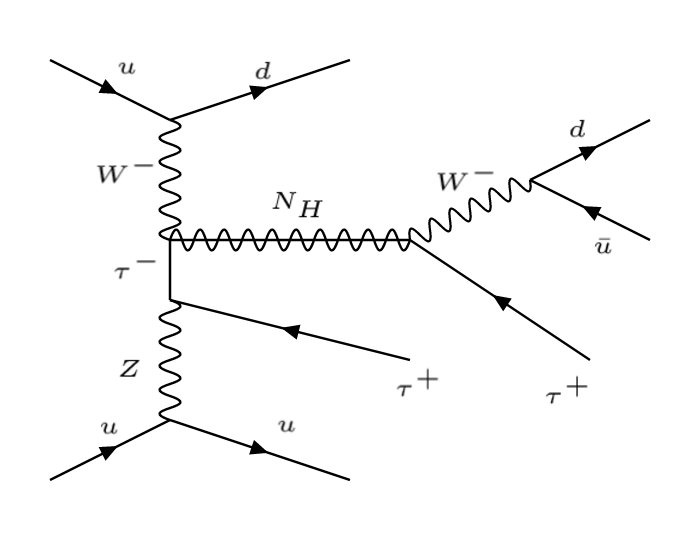
\includegraphics[scale = 0.45]{Figures/Feynman_hnZ}
\caption{Feynman diagram of simulated process involving Z boson}
\label{fig: hnZ}
\end{figure}

Figures \ref{fig: hnZ} and \ref{fig: hnGamma} show two of the main possible diagrams generated by MadGraph for the processes simulated. This two diagrams present a complete picture involving the processes shown in the diagrams of Figures \ref{fig: VBF} and \ref{fig: W}. Figure \ref{fig: VBF} shows the diagram of the vector boson fusion process, ocurring in Figures \ref{fig: hnZ} and \ref{fig: hnGamma} in the fusion of the W boson with the Z boson and the photon ($\gamma$) respectively. In these last two diagrams, the decay of the of the W boson coincides with the one shown in Figure \ref{fig: W} for the decay of the W boson resulting in a heavy neutrino and a lepton, which in this case is a $\tau$.

\begin{figure}[H]
\centering
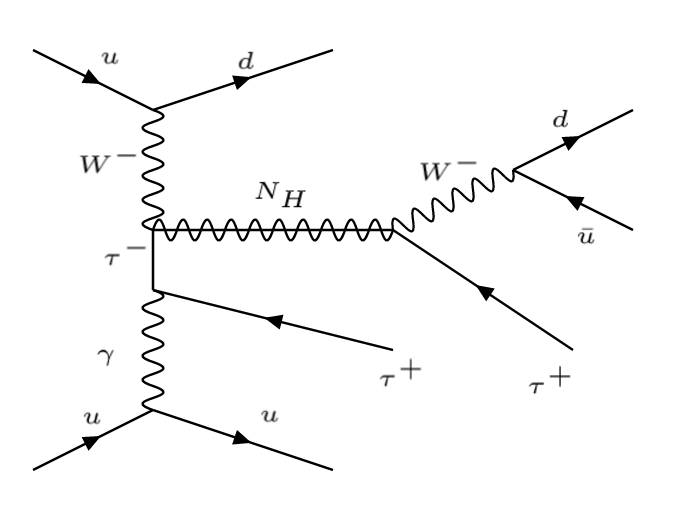
\includegraphics[scale = 0.45]{Figures/Feynman_hnGamma}
\caption{Feynman diagram of simulated process involving photon}
\label{fig: hnGamma}
\end{figure}

The simulation was performed in 10 different simulation batches each one containing 10,000 events. Every batch was generated with a different random seed to guarantee the independence of the events between each one of the generated batches. This independance was necessary because the 10,000 event files were merged to form a single file with 100,000 events. As explained earlier, after the events were simulated in MadGraph they were passed to Pythia and then to Delphes so the signal resembled one that could be found at CMS.  


\section{Definitions} \label{sec:definitions}

\subsection{Variable Definitions}

The transverse momentum or $p_{T}$, is defined as the momentum component that a particle has in the plane perpendicular to the beam line. In the coordinate system of the LHC, this plane corresponds to the $x-y$ plane.

The variable related with the polar angle in the LHC is called pseudorapidity, or $\eta$, defined as in Equation \ref{eq: eta}. The use of this variable is justified for mainly two reasons. The first one is that $\Delta \eta$, contrary to $\Delta \theta$, is a Lorentz invariant. This makes $\Delta \eta$ a more natural variable than $\Delta \theta$ for relativistic calculations. The second reason is that the distribution of the values of $\eta$ in barrel region, where the multiplicity of particle is less than in the end-caps, is wider allowing the $\eta$ particle distribution to be aproximately constant.

\begin{equation}
 \eta = -\ln\left[\tan\left(\frac{\theta}{2}\right)\right]
 \label{eq: eta}
\end{equation}

In the preliminary analysis of the variable distributions shape using normalized to the unit plots, i.e. the area under the distribution for the distribution is equal to one, a separation between signal and background was achieved in the transverse momentum variable of both jets and taus. However, in distribution involving all the cuts considered fothe analysis, the separation noticeable but considerably smaller. The separation between background and signal was bigger for the tau transverse momentum $p_{T}(\tau)$ than the one shown by both leading and sub-leading jets.

With the idea of exploiting the small but existent different between signal and background in the $p_{T}$ varibles, two new variables shown in Equations \ref{eq: HT} and \ref{eq: ST} were created to check for possible further separation between signal and background. As shown in equation \ref{eq: HT}, the $H_{T}$ variable is defined as the scalar sum of the jets with $p_{T}$ greater than 30 GeV and $|\eta| < 5$ that are not B-jets. $S_{T}$ is defined as the scalar sum of jets that fullfilll the same conditions of $H_{T}$, added to the $p_{T}$ of the $\tau$'s in the event.

Since the $\tau$ selection is important for this analysis, it is relevant to provide a further description of the selection criteria for the $\tau$'s in the simulated events. For starters, a jet identified as a tau is considered a valid $\tau$ if it has minimum a transverse momentum of 20 GeV. Also, it was required that a valid $\tau$ should not overlap with an electron or a muon. That is, the $\Delta R$, defined as $\Delta R = \sqrt{(\Delta \eta)^2 + (\Delta \phi)^2}$ should not be less than 0.3. This condition guarantees that the jet identified as a $\tau$ does not overlap with other leptons. Other condition required for a valid $\tau$ is that the jet has a minimum transverse momentum of 20 GeV. Since the final state for this analysis includes two $tau$'s, the two taus with greater $p_{T}$ are selected among a maximum of three taus stored for each event. The leading $\tau$ is the one with highest $p_{T}$ and the sub-leading $\tau$ is the one with second highest $p_{T}$.

\begin{equation}
 H_{T} = \sum_{i=1}^{n} p_{T}(jet_{i})
 \label{eq: HT}
\end{equation}

\begin{equation}
 S_{T} = \sum_{i=1}^{n} p_{T}(jet_{i}) + \sum_{j=1}^{m} p_{T}(\tau_{j})
 \label{eq: ST}
\end{equation}

\subsection{Cut Definitions}

In order to achieve a separation between background and signal, several successive cuts in variables were made. This section contains a list of the cuts with its explanation. 

\chapter{Distribution Analysis} \label{sec: disanalysis}

\section{Normalized Distributions}

The normalized plots are useful to check the shape of backgrounds and signal distributions. These shapes help to identify which variables are not useful for the analysis because the backgrounds overlap with the signal and which variables have to be studied with greater detail because the signal separates from the backgrounds from certain points. An example for both cases is provided in Figures \ref{fig: tau2etaunitNC} and \ref{fig: tau1ptunitNC}. In figure \ref{fig: tau2etaunitNC} it can be seen that the signal overlaps for all values with the background distributions. That is why this plot can be used to conclude that the $\eta$ variable from the sub-leading $\tau$ is not useful to isolate the signal from the background. In contrast, the plot in Figure \ref{fig: tau1ptunitNC} show that from around 150 GeV the signal separates from the background distributions. This separation for the $p_{T}$ of the leading $\tau$ suggests that this variable should be examined more closely through the subsequent cuts. 

\begin{figure}
\centering
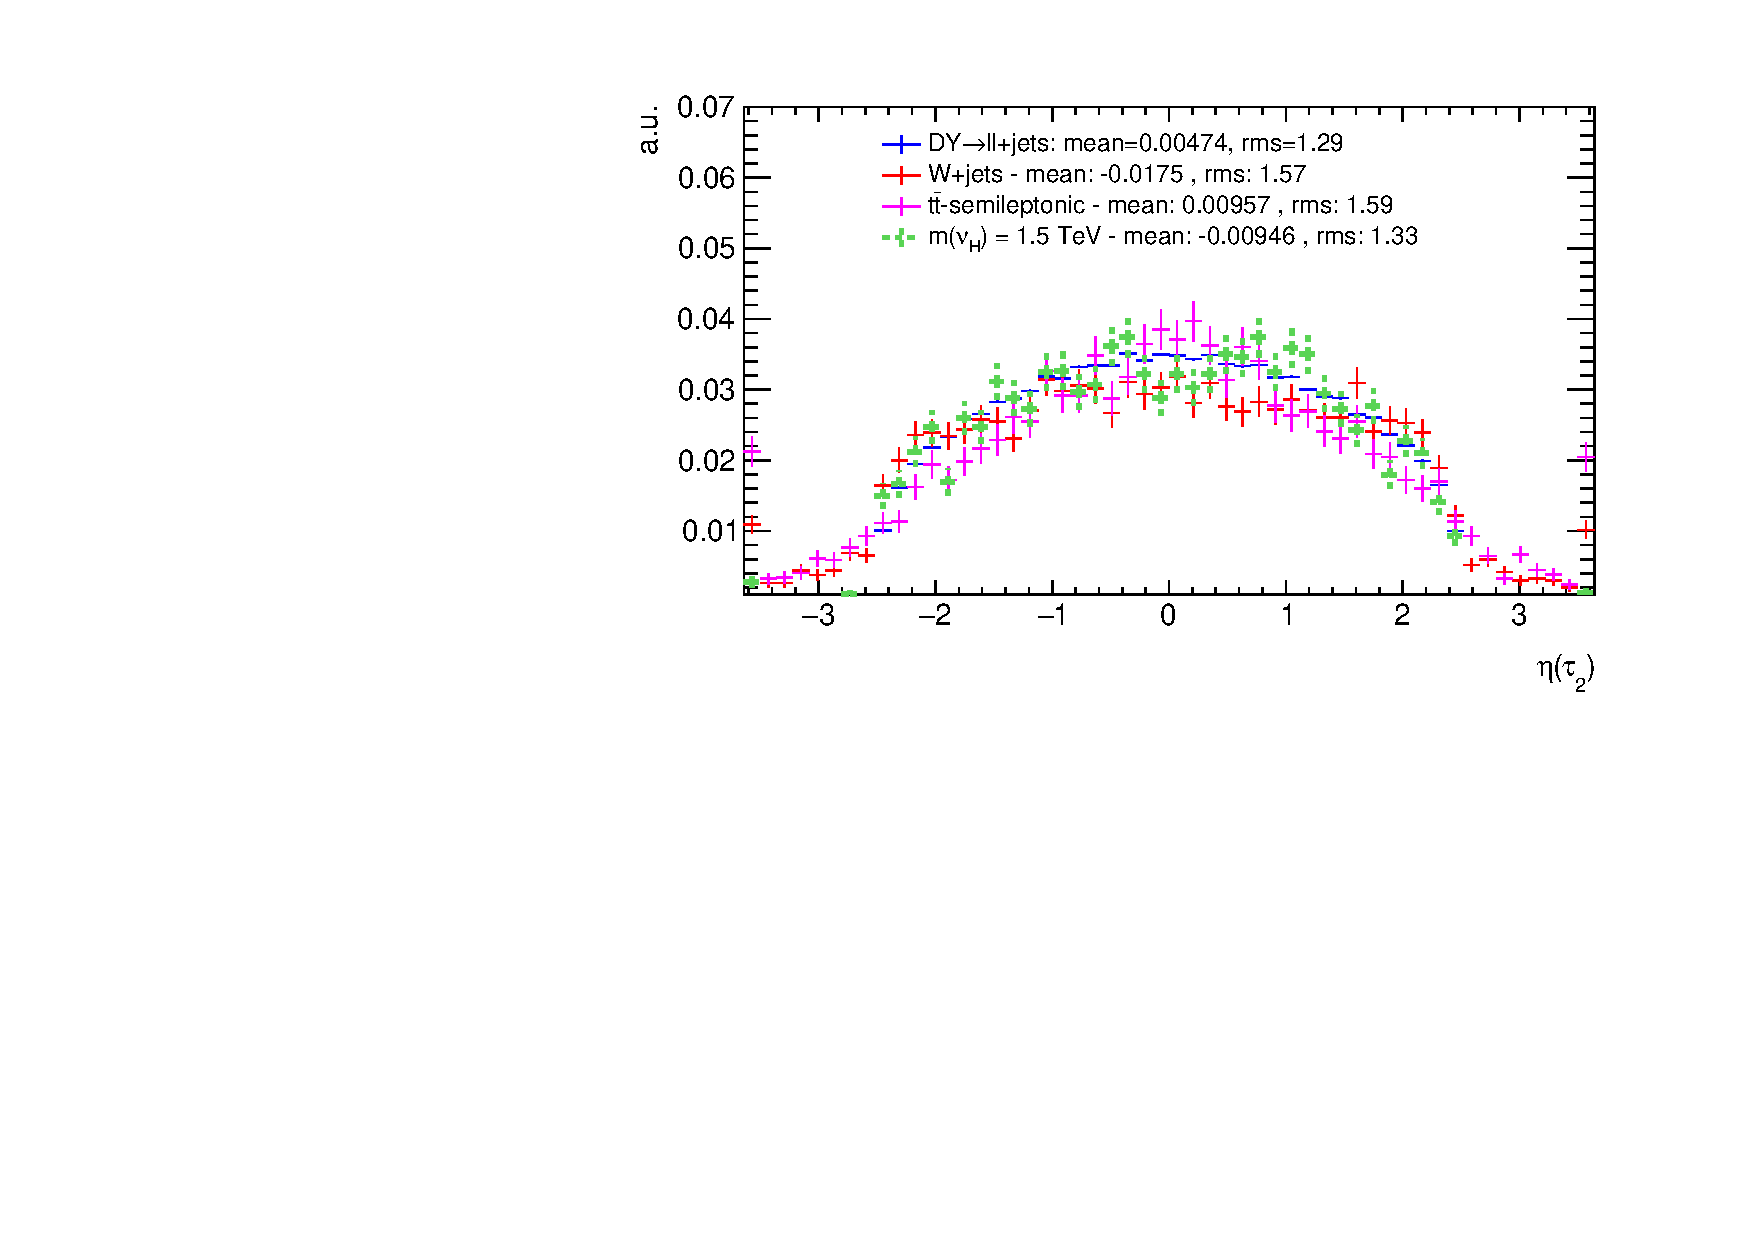
\includegraphics[width=\linewidth]{Figures/Plots/tau2_eta_unitNC.pdf}
\caption{Unit plot of $\eta$ from the sub-leading $\tau$ with no cuts}
\label{fig: tau2etaunitNC}
\end{figure}

\begin{figure}
\centering
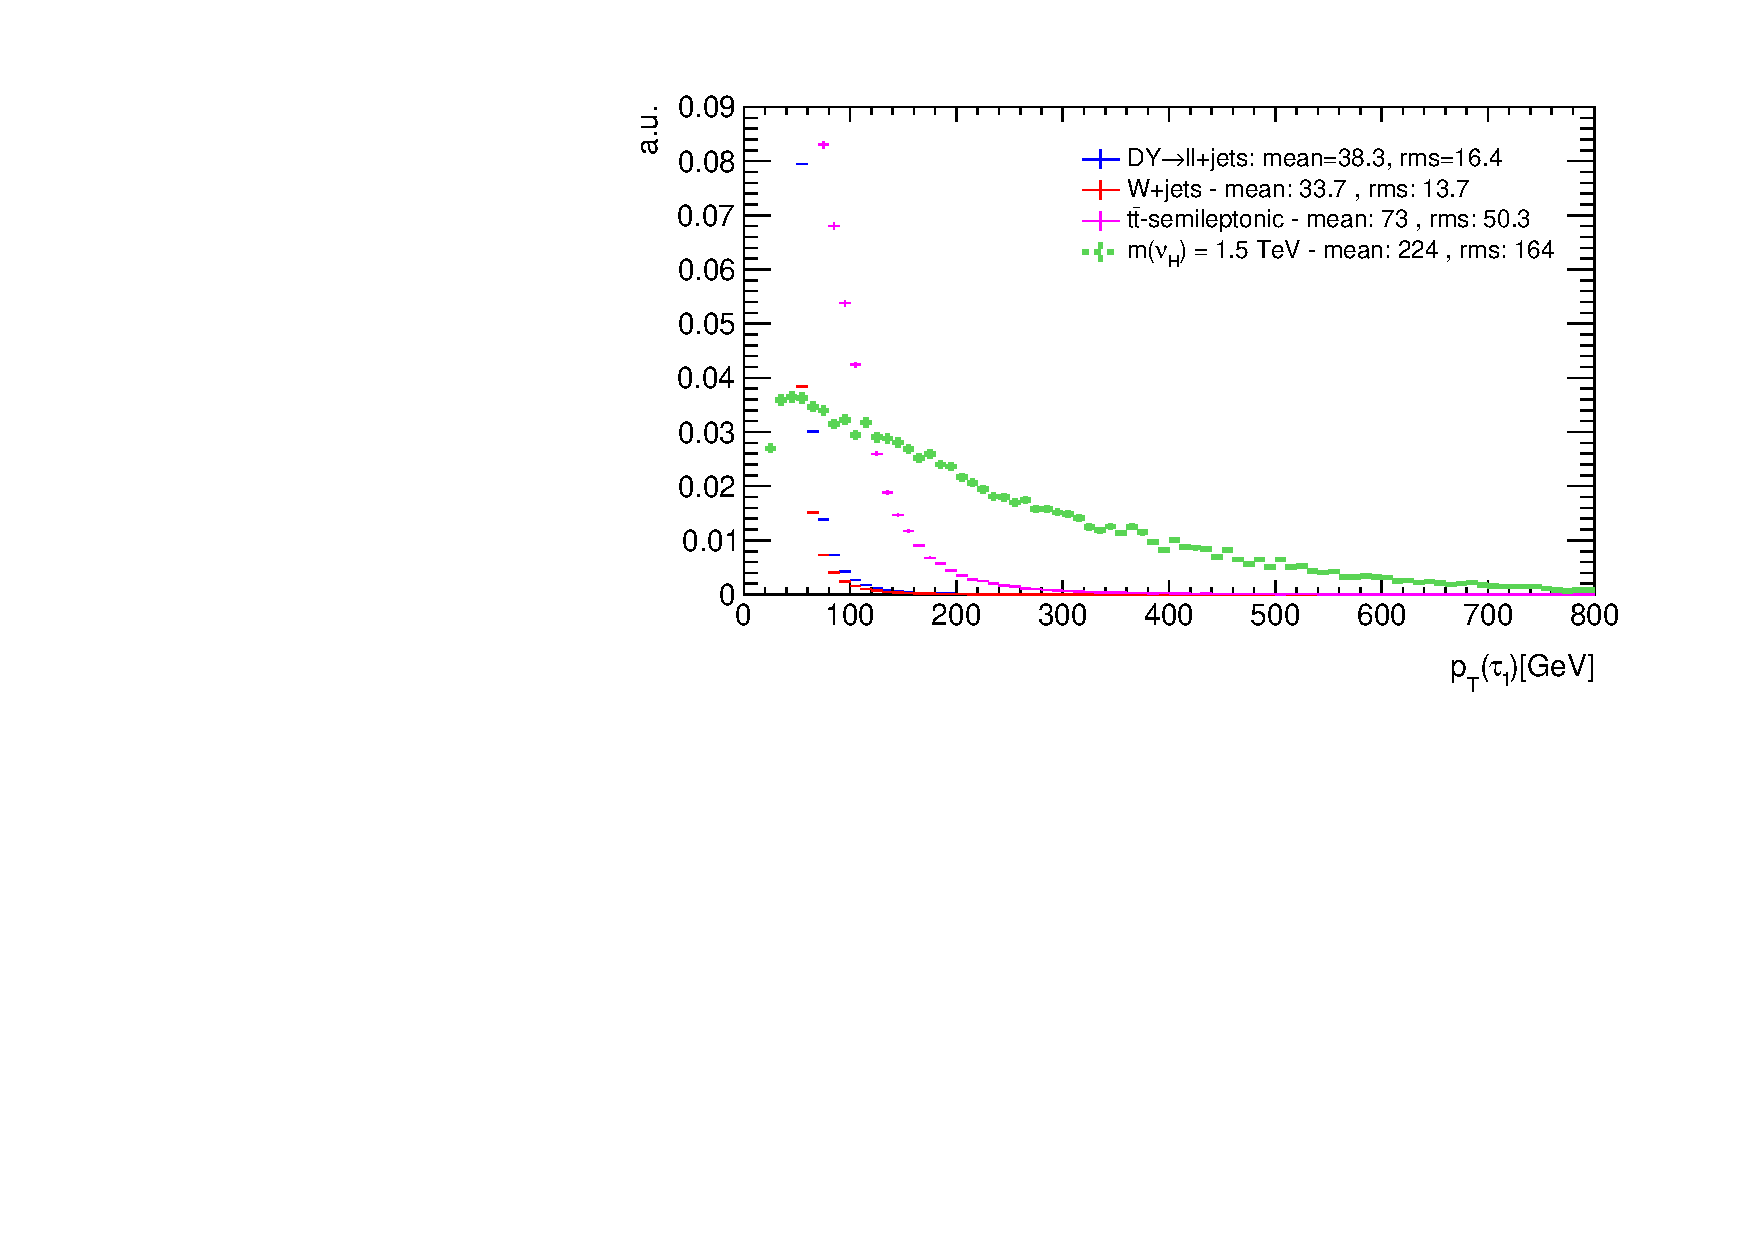
\includegraphics[width=\linewidth]{Figures/Plots/tau1_pt_unitNC.pdf}
\caption{Unit plot of $p_{T}$ of leading $\tau$ with no cuts}
\label{fig: tau1ptunitNC}
\end{figure}

To understand the definition of $H_{T}$ and $S_{T}$ mentioned in chapter \ref{sec:definitions}, the plots in Figure \ref{fig: ptUnitPlots} are shown. The four plots show a separation, in some cases a smaller than others, between the signal and backgrounds distributions. A tendency of the signal jets to have greater transverse momentum than the ones in the backgrounds is shown. This tendency is also displayed for both $\tau$'s. Hence, the distributions of $H_{T}$ and $S_{T}$ should show a similar behaviour because this variables are the result of adding the transverse momentum of jets and $\tau$'s in the event.

\begin{figure}       
        \centering
        \begin{subfigure}[b]{0.475\textwidth}
            \centering
            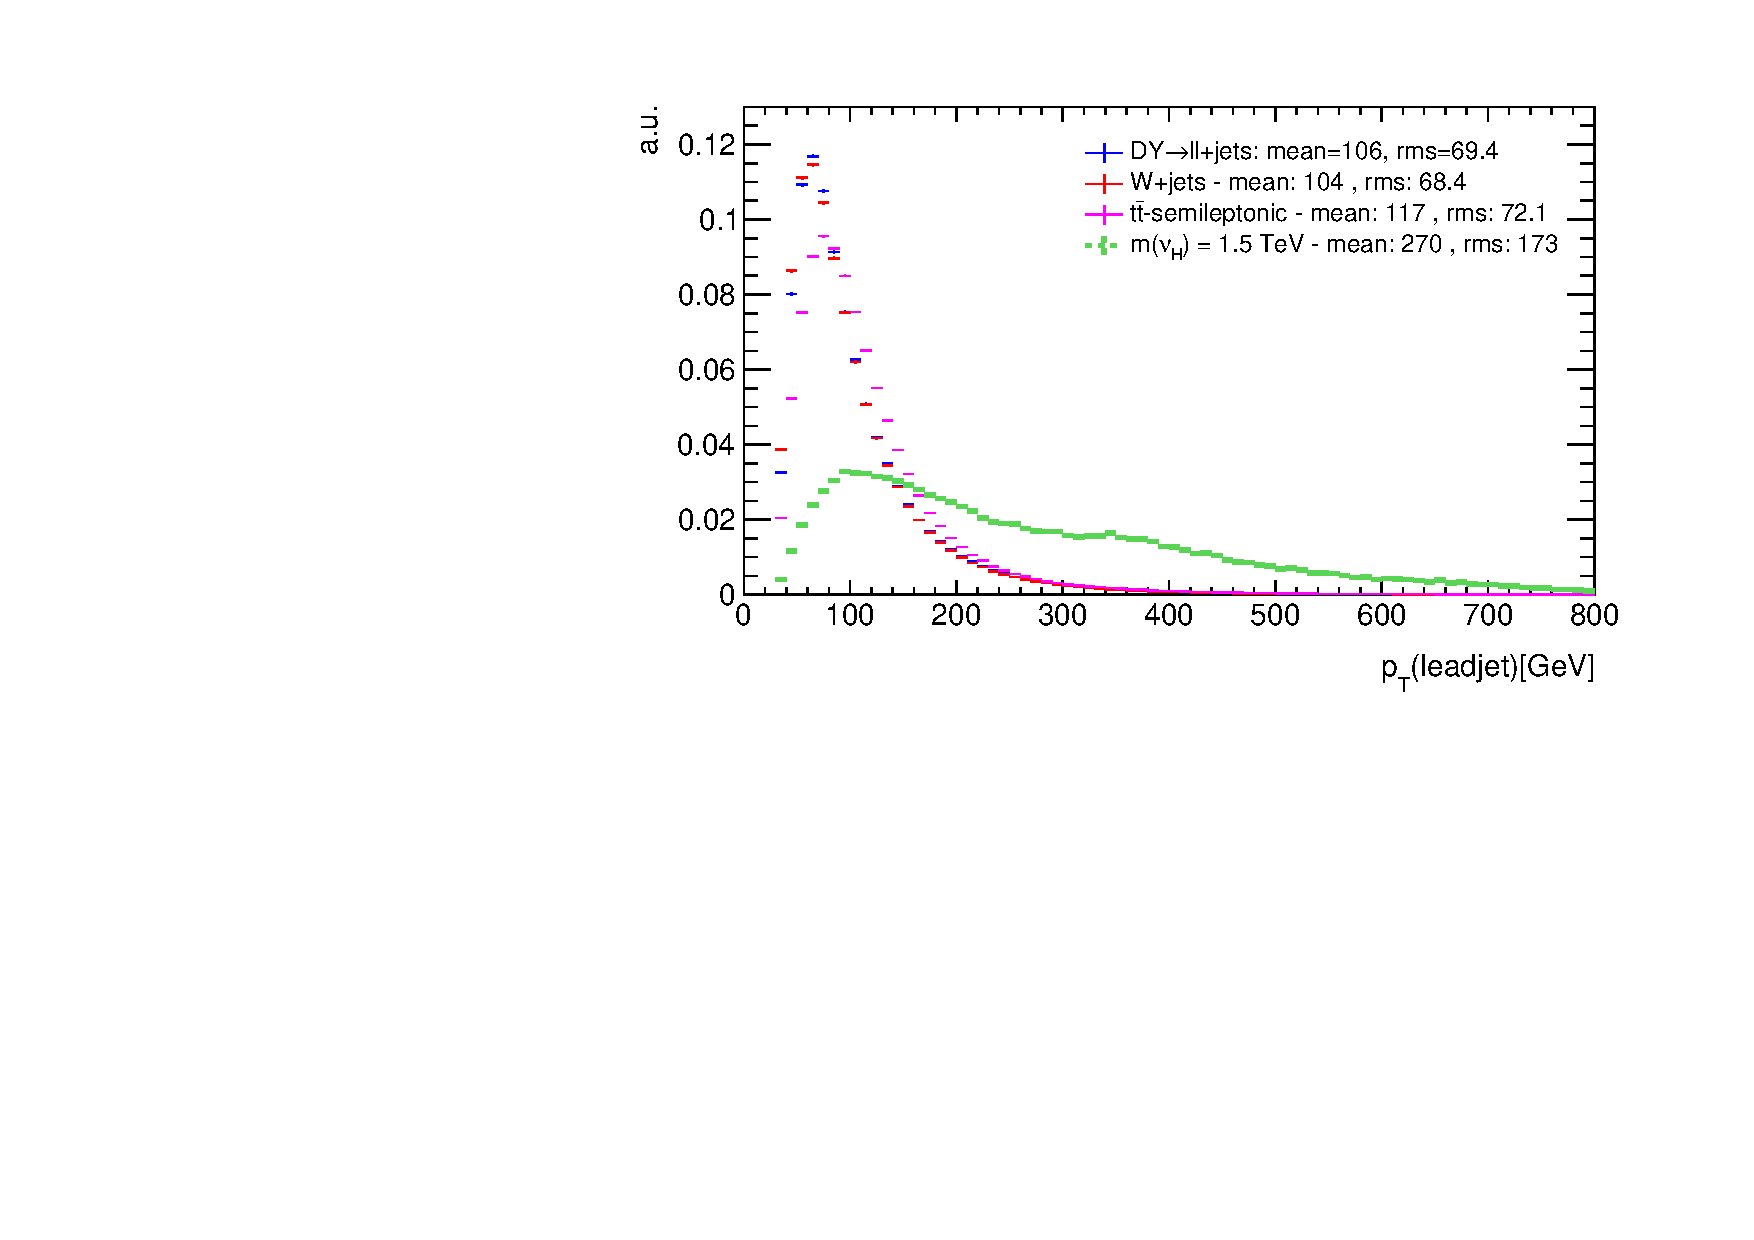
\includegraphics[width=\textwidth]{Figures/Plots/ljet_pt_unitNC}
            \caption[]%
            {{\small Leading jet $p_{T}$ unit plot}}    
            %\label{fig:mean and std of net14}
        \end{subfigure}
        \hfill
        \begin{subfigure}[b]{0.475\textwidth}  
            \centering 
            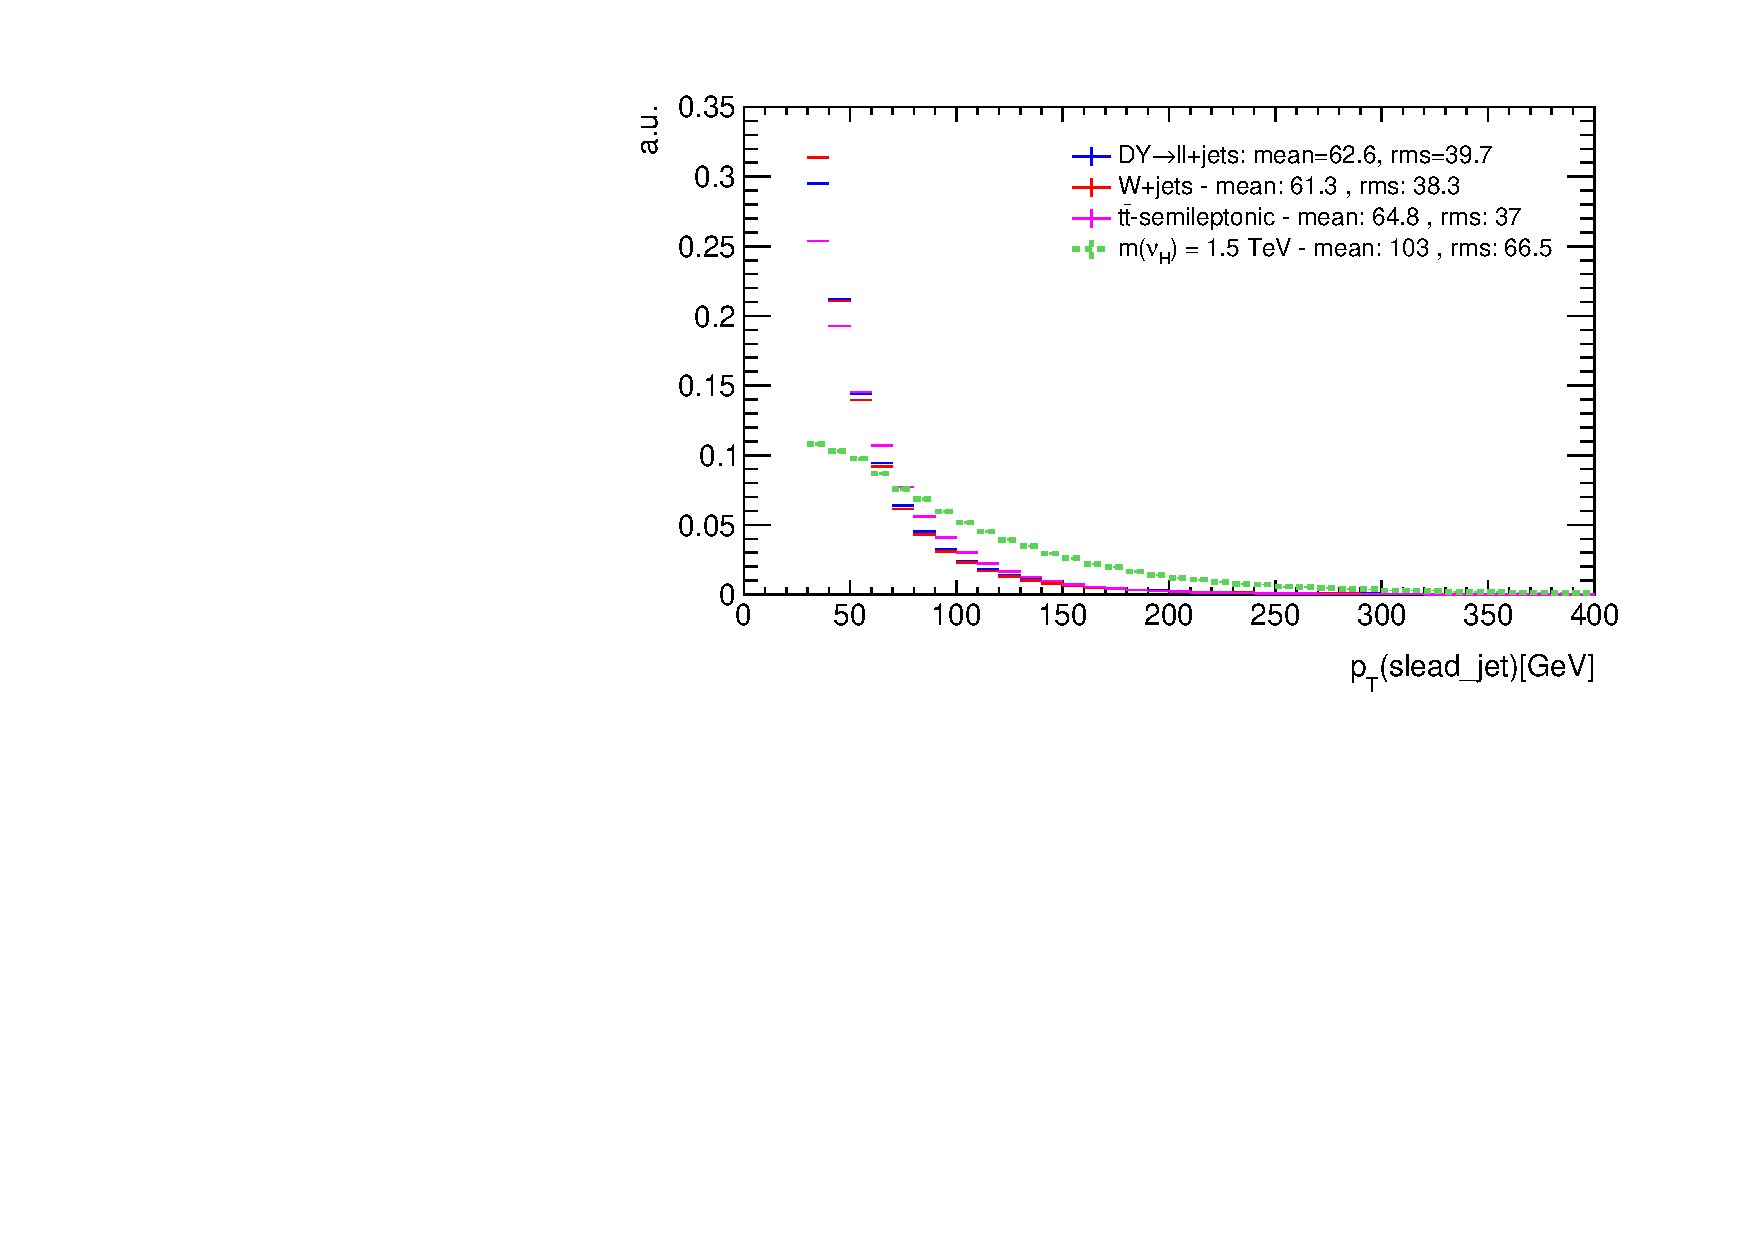
\includegraphics[width=\textwidth]{Figures/Plots/sjet_pt_unitNC}
            \caption[]%
            {{\small Sub-leading jet $p_{T}$ unit plot}}    
            %\label{fig:mean and std of net24}
        \end{subfigure}
        \vskip\baselineskip
        \begin{subfigure}[b]{0.475\textwidth}   
            \centering 
            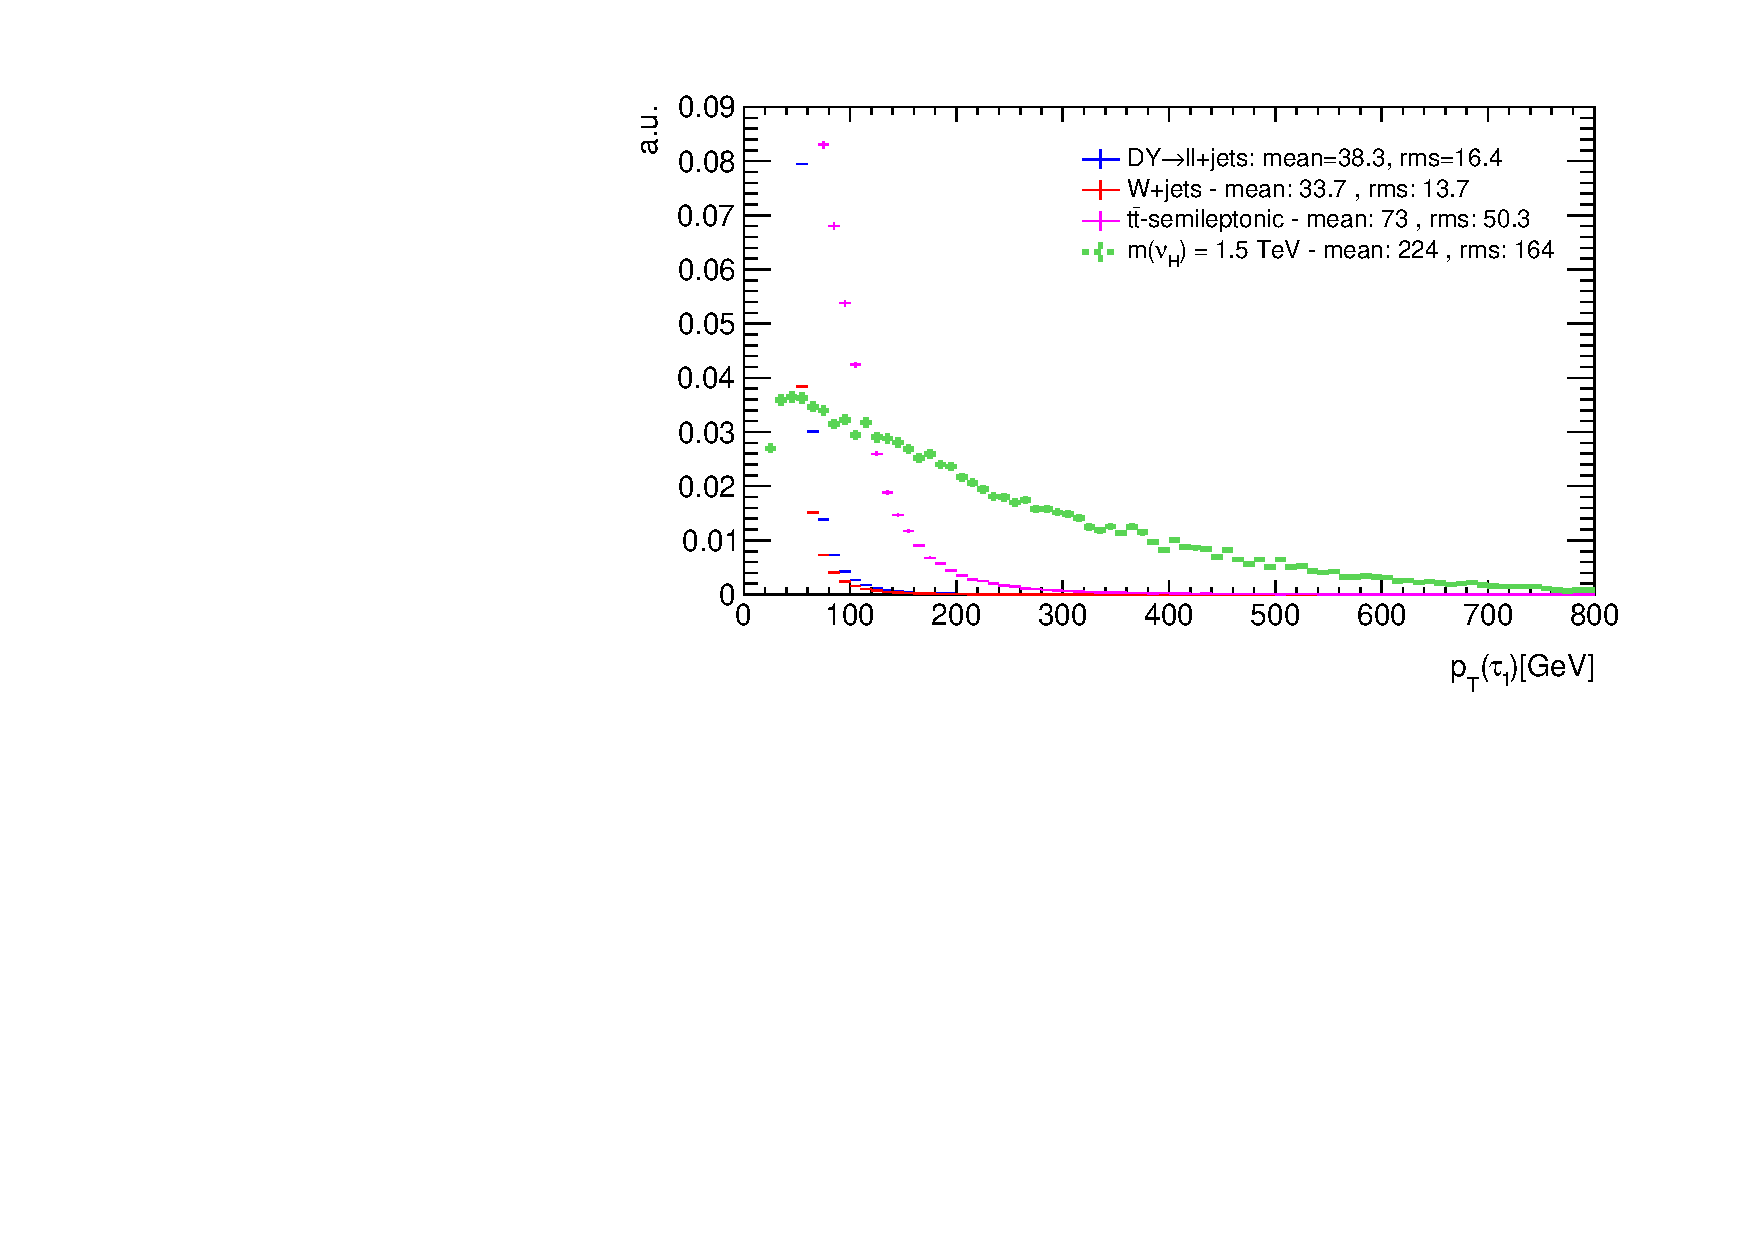
\includegraphics[width=\textwidth]{Figures/Plots/tau1_pt_unitNC}
            \caption[]%
            {{\small Leading $\tau$ $p_{T}$ unit plot}}    
            %\label{fig:mean and std of net34}
        \end{subfigure}
        \quad
        \begin{subfigure}[b]{0.475\textwidth}   
            \centering 
            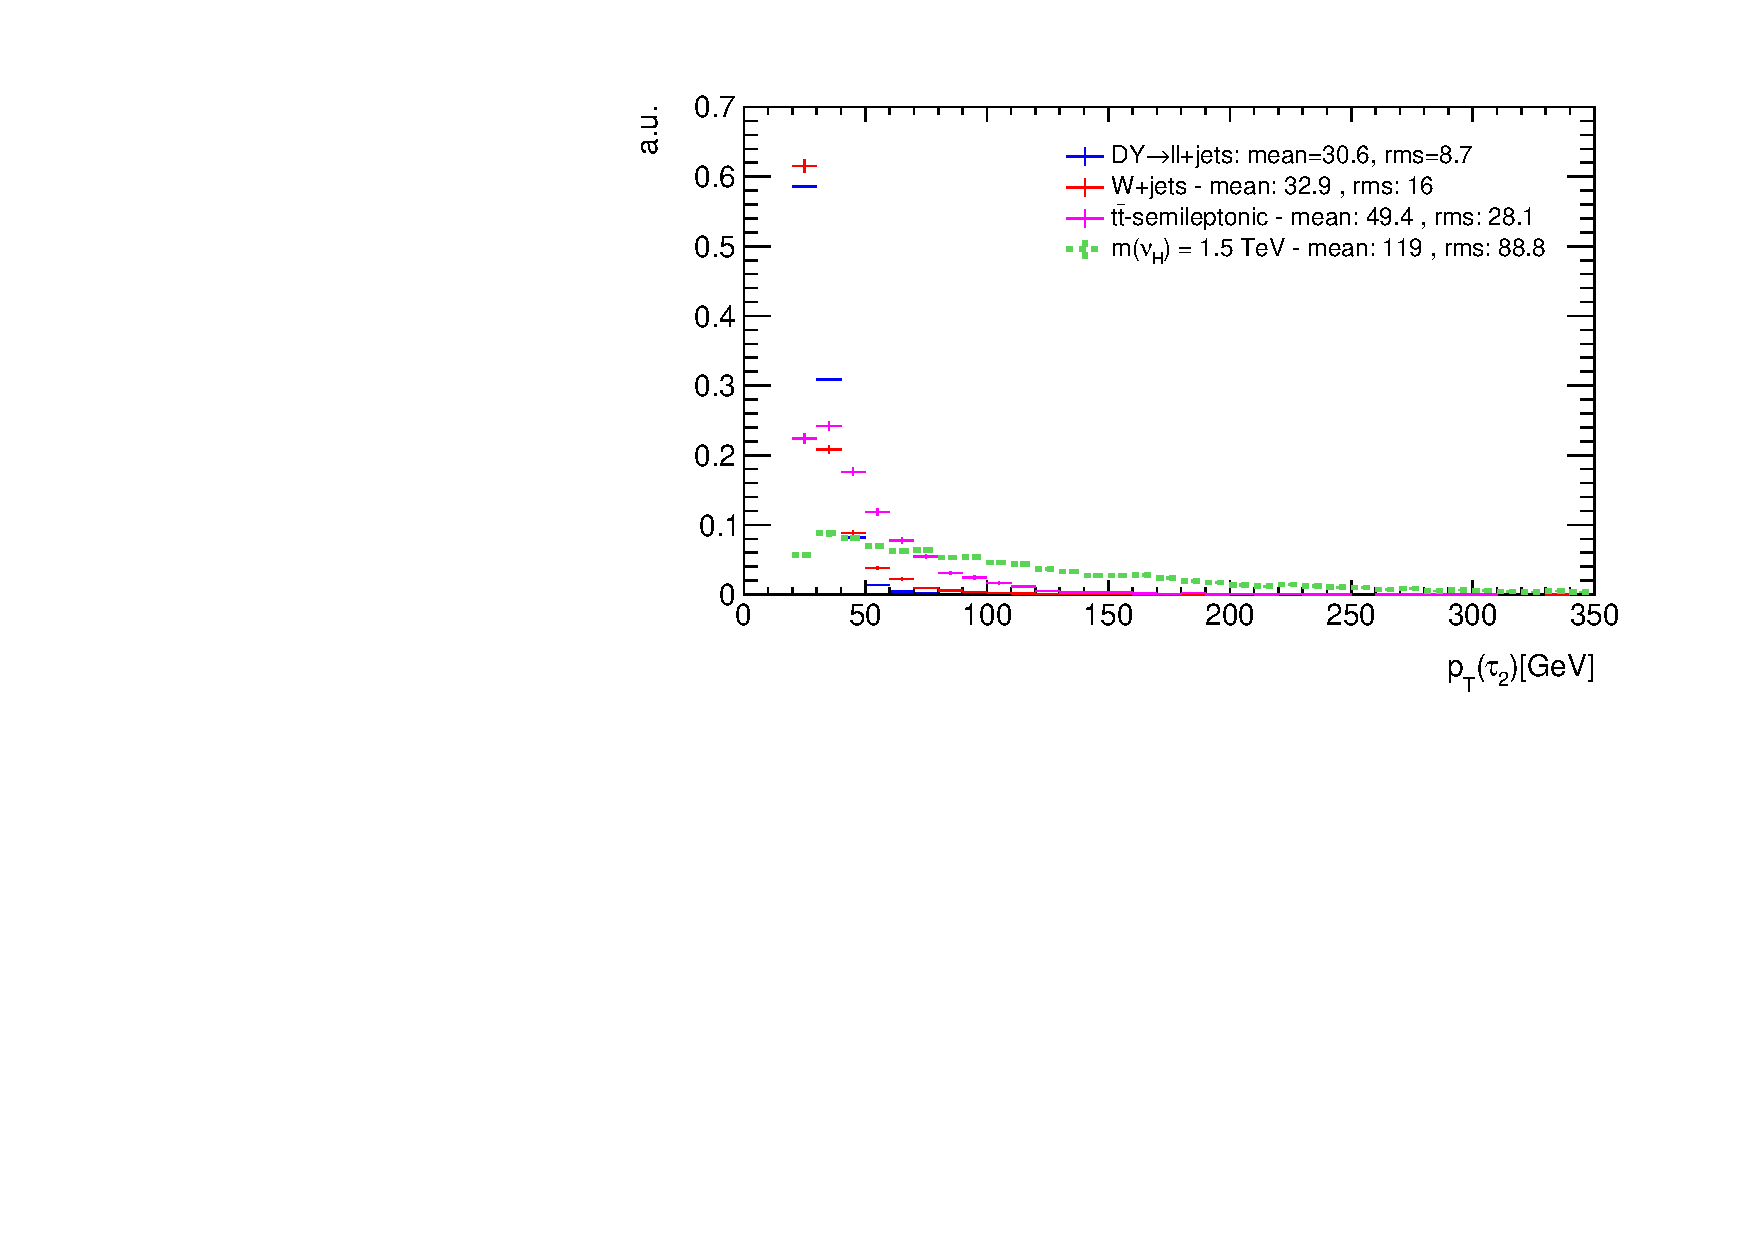
\includegraphics[width=\textwidth]{Figures/Plots/tau2_pt_unitNC}
            \caption[]%
            {{\small Sub-leading $\tau$ $p_{T}$ unit plot}}    
            %\label{fig:mean and std of net44}
        \end{subfigure}
        \caption[ $p_T$ unit plots for different bodies in the event]
        {\small $p_T$ unit plots for different bodies in the event} 
         \label{fig: ptUnitPlots}
\end{figure}

In Figures \ref{fig: HTunitNC} and \ref{fig: STunitNC}, the normalized plots with no cuts of $H_{T}$ and $S_{T}$ are shown. It can be seen that indeed a greater separation between signal and background was achieved. Unlike the distributions of the $\tau$'s and jets transverse momentum, the maxima of $H_{T}$ and $S_{T}$ lie outside the backgrounds distributions. Furthermore, the background that overlaps at a greater energy with the signal corresponds to $t\bar{t}$. Taking into account what was mentioned in section \ref{sec: cutdefinitions}, the overlap between the signal and this background could be reduced with the cut related with the number of B-jets in the event. This is why this two variables need to be studied closer in the analysis.

\begin{figure}
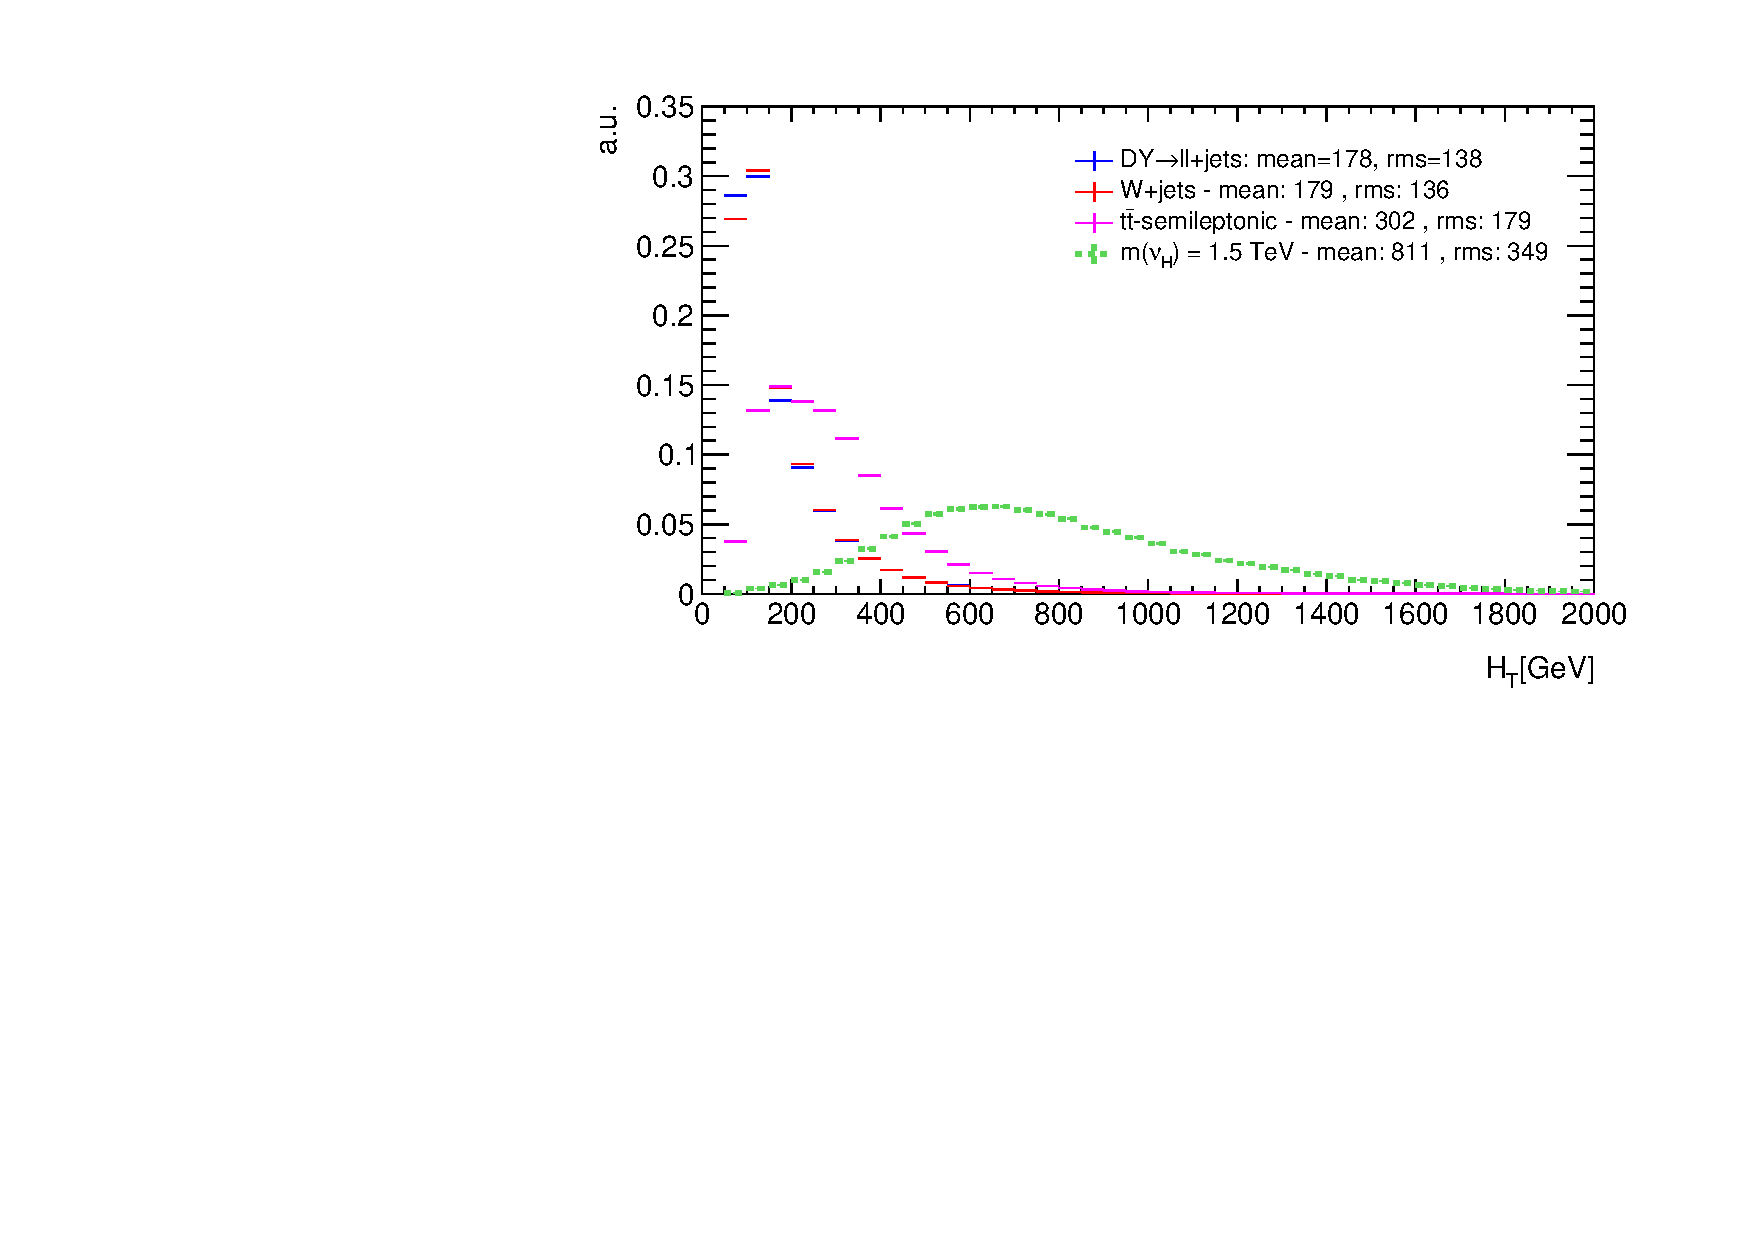
\includegraphics[width=\linewidth]{Figures/Plots/HT_unitNC.pdf}
\caption{Unit plot of $H_{T}$ with no cuts}
\label{fig: HTunitNC}
\end{figure}

\begin{figure}
\centering
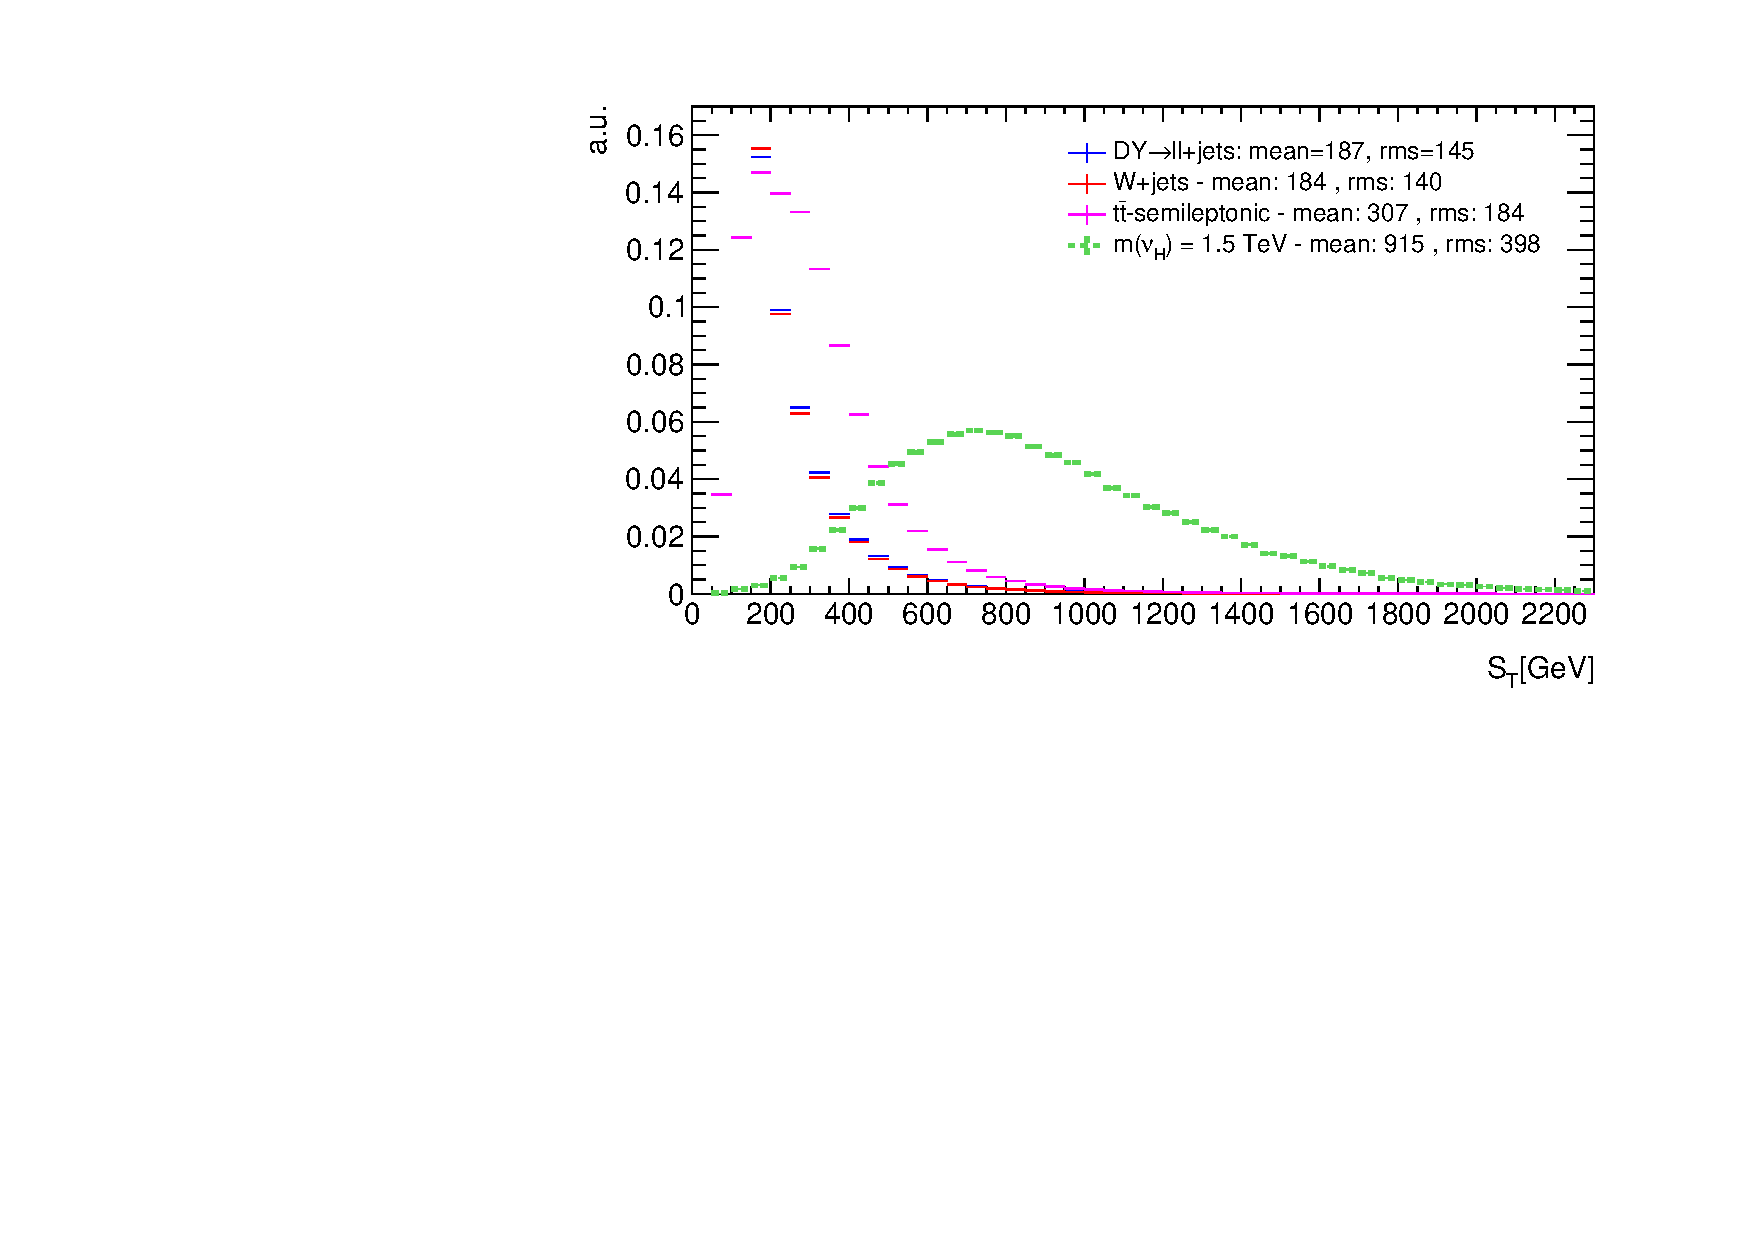
\includegraphics[width=\linewidth]{Figures/Plots/ST_unitNC.pdf}
\caption{Unit plot of $S_{T}$ with no cuts}
\label{fig: STunitNC}
\end{figure}

In Figures \ref{fig: HTunitVBF} and \ref{fig: STunitVBF}, the plots incuding cuts of $H_{T}$ and $S_{T}$ respectively are shown. Both plots include all the cuts mentioned in section \ref{sec: cutdefinitions}. A rebining of the histograms was necessary, because due to the cuts, the number of backgrounds events decreased significantly. This made the error bars for these histograms larger making the analysis of the plot more difficult. For that reason, a bin size of 400 GeV was defined for both of these plots. Comparing the two signal histograms, it can be seen that the maximum of the $H_{T}$ distribution still overlaps with the background distributions. Although the signal in this case appears on top of the background, it has to be noted that this normalized plots are only useful to get an idea of the distribution shapes. That is why the fact the the signal appears on top of the background does not mean that the signal can be detected over the background for this value. On the contrary, the maximum of the $S_{T}$ signal distribution has its maximum when the background distributions start to decay. This distribution shape  difference between $H_{T}$ and $S_{T}$ is related with the fact that the signal has $\tau$'s with higher $p_{T}$ than the ones found in the backgrounds.

\begin{figure}
\begin{center}
 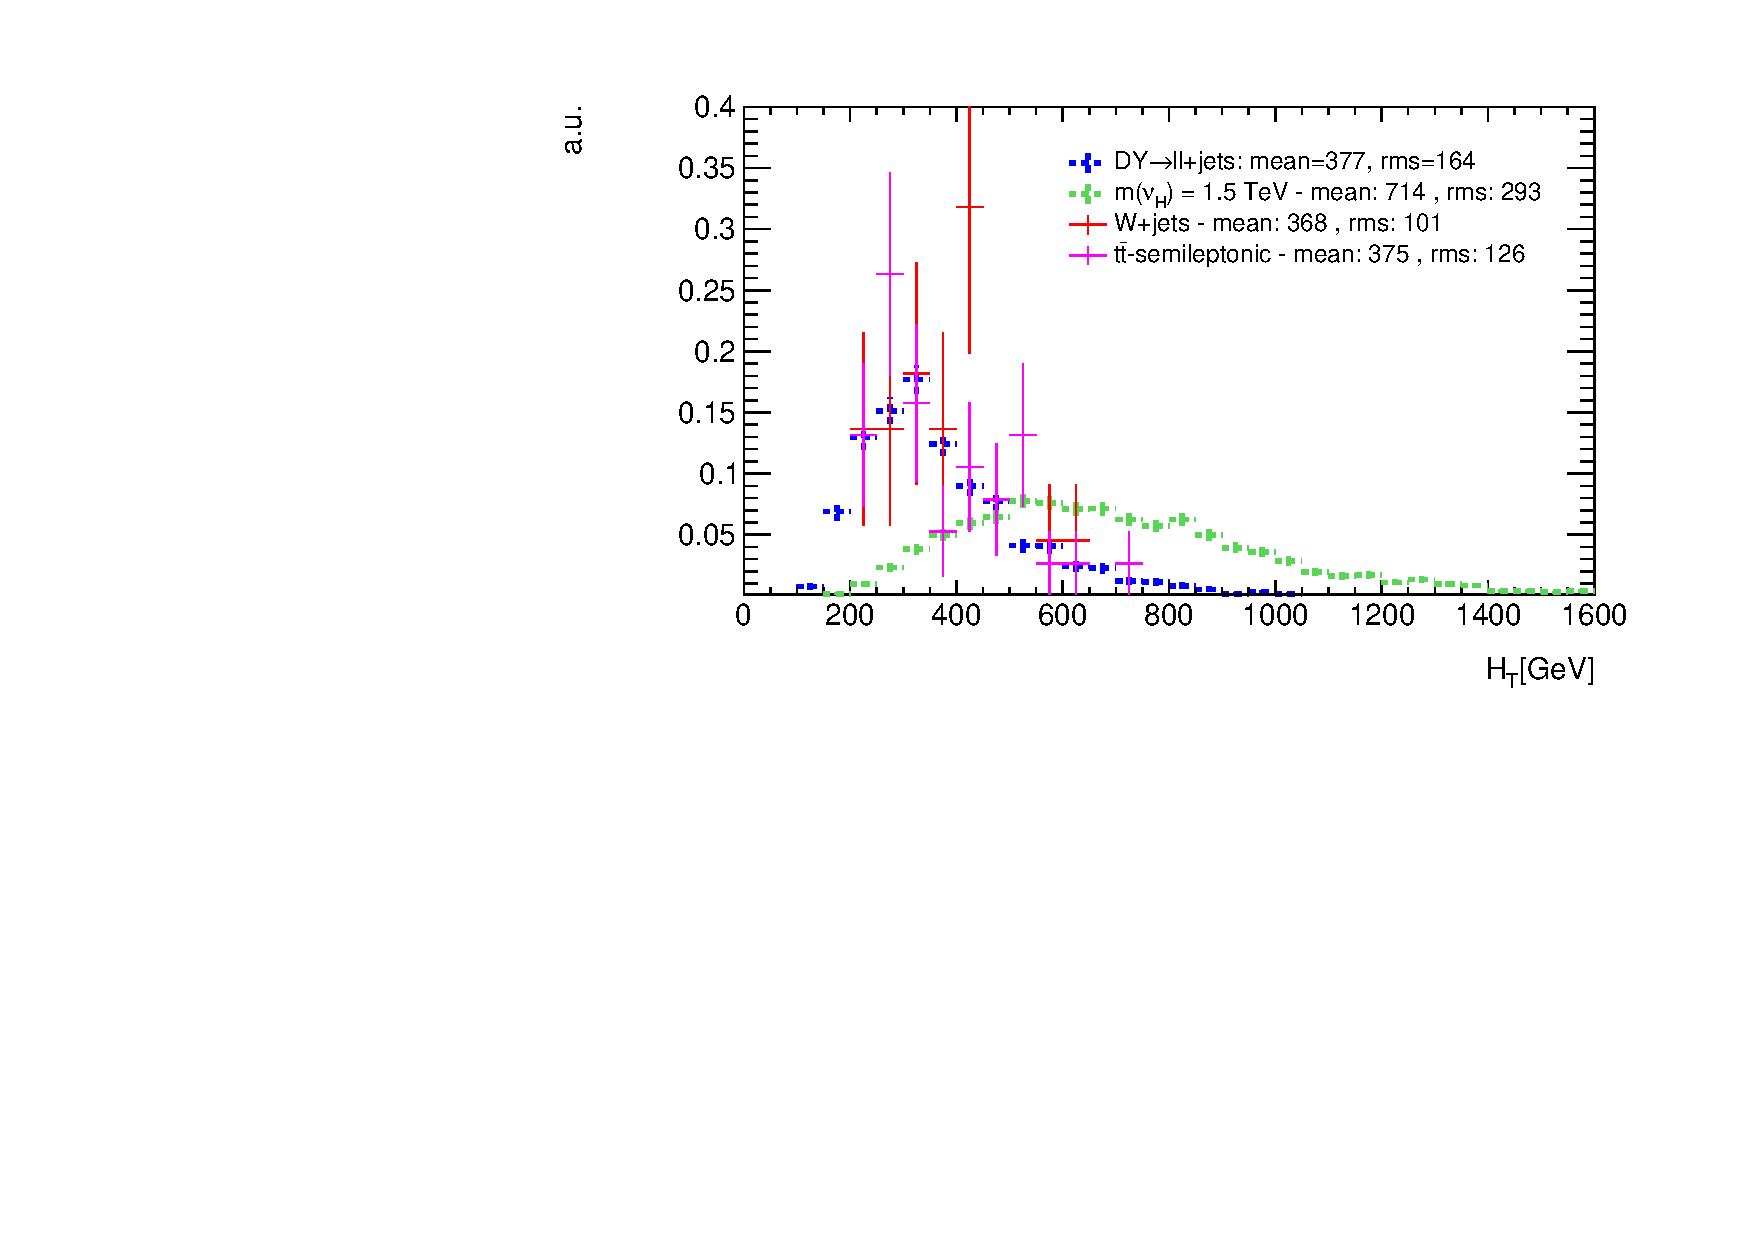
\includegraphics[width=\linewidth]{Figures/Plots/HT_unitVBF.pdf}
\end{center}
\caption{Unit plot of $H_{T}$ with VBF cuts}
\label{fig: HTunitVBF}
\end{figure}

\begin{figure}
\centering
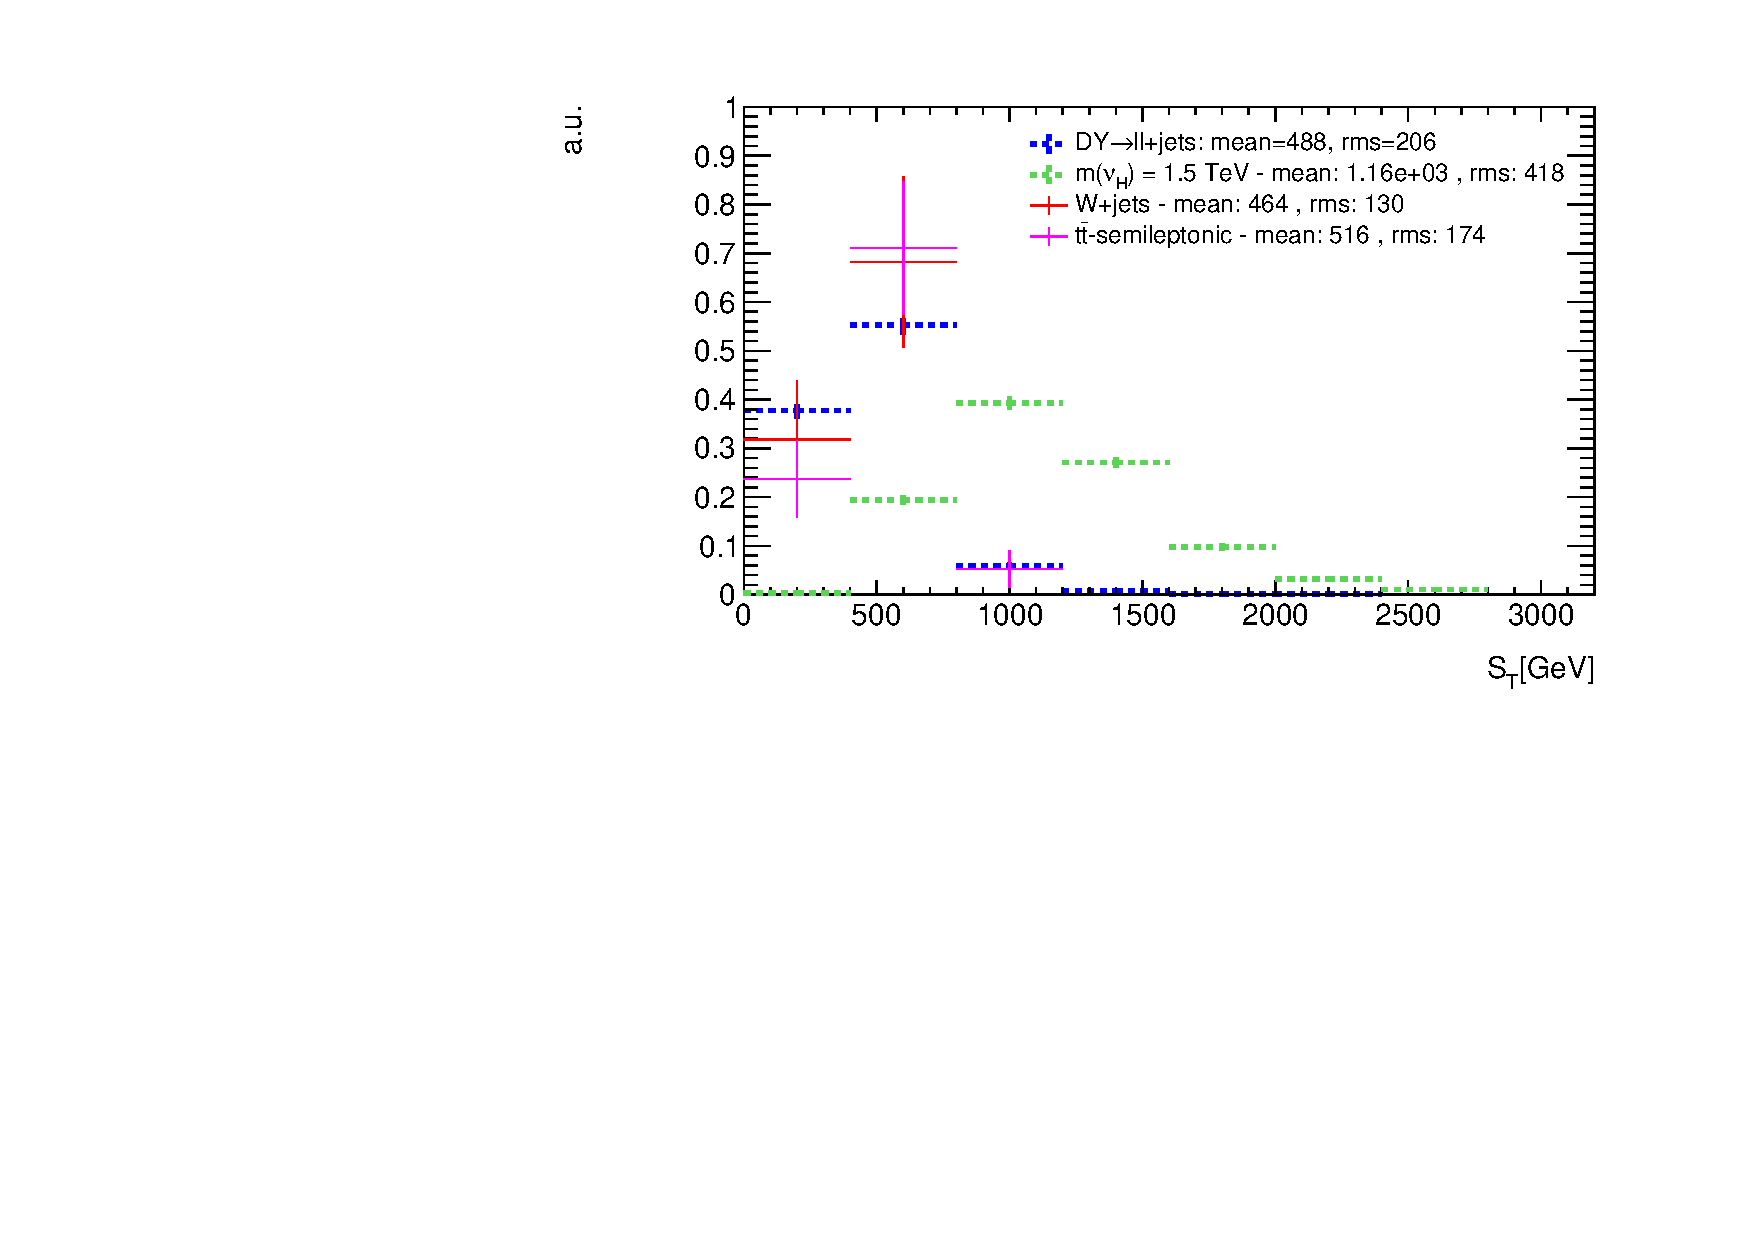
\includegraphics[width=\linewidth]{Figures/Plots/ST_unitVBF.pdf}
\caption{Unit plot of $S_{T}$ with VBF cuts}
\label{fig: STunitVBF}
\end{figure}

The mean values for $S_{T}$ shown in Figures \ref{fig: STunitNC} and \ref{fig: STunitVBF} are 915 GeV and 1160 GeV respectively. From the Feynman diagram in Figure \ref{fig: hnGamma}, it can be seen that the jets in the event and one of the taus come from the heavy neutrino decay. Taking into account that the defined mass for the heavy neutrino is 1.5 TeV, it is expected that the maximum of the $S_{T}$ distribution is around this value. This analysis leads to the conclusion that the cuts made to the histograms are helping to select the significant events, because the mean $S_{T}$ is closer to the expected value after performing all the cuts.








%----------------------------------------------------------------------------------------
%	APÉNDICES
%----------------------------------------------------------------------------------------

%\addtocontents{toc}{\vspace{2em}} % Agrega espacios en la toc

%\appendix % Los siguientes capítulos son apéndices

%  Incluye los apéndices en el folder de apéndices

%\include{Apendices/Ap}
%\thispagestyle{empty}
%\include{Apendices/AppendixB}
%\include{Apendices/AppendixC}

%\addtocontents{toc}{\vspace{2em}} % Agrega espacio en la toc


%----------------------------------------------------------------------------------------
%	BIBLIOGRAFÍA
%----------------------------------------------------------------------------------------
%\backmatter
%\nocite{*}
%\bibliographystyle{plain}
%\bibliography{bibliografía.bib} %Aquí ponen el nombre del archivo .bib


\begin{thebibliography}{10}

\bibitem {Detectores}Particle Data Group, Olive, K. A. et al. , Chin.Phys. C38, 090001 (2014)


\bibitem{Super-Kamiokande} Fukuda, S. et al. (2003) Nuclear Instruments and Methods in Physics Research A 501 (2003) 418–462

\bibitem{KamLAND} Decowski, M. (2016). KamLAND's precision neutrino oscillation measurements. Nuclear Physics B, 908, pp.52-61.

\bibitem{K2K} K2K Collaboration: Aliu, E. et al (2005). Evidence for Muon Neutrino Oscillation in an Accelerator-Based Experiment. Physical Review Letters, 94(8).

\bibitem {Experimentos}Nakamura, K. et al. (2010) (Particle Data Group), J. Phys. G 37, 075021 (2010) 

\bibitem {See-saw} Deppisch, F., Bhupal Dev, P., \& Pilaftsis, A. (2015). Neutrinos and collider physics. New Journal Of Physics, 17(7), 075019. http://dx.doi.org/10.1088/1367-2630/17/7/075019

\bibitem {LEP} Abdesslam, A. et al. (2014) Type II Seesaw Higgsology and LEP/LHC constraints. arXiv:1411.5645 [hep-ph]

\bibitem {CMS ATLAS} Khachatryan, V., Sirunyan, A., Tumasyan, A., Adam, W., Asilar, E., \& Bergauer, T. et al. (2016). Search for heavy Majorana neutrinos in $e\pm e\pm +$ jets and $e\pm$ $\mu \pm +$ jets events in proton-proton collisions at s = 8 $\sqrt{s}=8$ TeV. Journal Of High Energy Physics, 2016(4).

\bibitem {VBF Search} Brooke, J., Buckley, M., Dunne, P., Penning, B., Tamanas, J., \& Zgubič, M. (2016). Vector boson fusion searches for dark matter at the LHC. Physical Review D, 93(11). http://dx.doi.org/10.1103/physrevd.93.113013

\bibitem{MadGraph} Alwall, J., Herquet, M., Maltoni, F., Mattelaer, O., \& Stelzer, T. (2011). MadGraph 5: going beyond. Journal Of High Energy Physics, 2011(6). http://dx.doi.org/10.1007/jhep06(2011)128

\bibitem{Pythia}Sjöstrand, T., Ask, S., Christiansen, J., Corke, R., Desai, N., \& Ilten, P. et al. (2015). An introduction to PYTHIA 8.2. Computer Physics Communications, 191, 159-177. http://dx.doi.org/10.1016/j.cpc.2015.01.024

\bibitem{Delphes} de Favereau, J., Delaere, C., Demin, P., Giammanco, A., Lemaître, V., Mertens, A., \& Selvaggi, M. (2014). DELPHES 3: a modular framework for fast simulation of a generic collider experiment. Journal Of High Energy Physics, 2014(2). http://dx.doi.org/10.1007/jhep02(2014)057

\bibitem{ROOT} Antcheva, I., Ballintijn, M., Bellenot, B., Biskup, M., Brun, R., \& Buncic, N. et al. (2009). ROOT — A C++ framework for petabyte data storage, statistical analysis and visualization.

\end{thebibliography}



\end{document}